\documentclass[useAMS,usenatbib]{mn2e}
\usepackage{myaasmacros}
\usepackage{graphicx}
\usepackage{ulem}
\usepackage{color}
\usepackage{amsmath}

% definitions of symbols
\def\ltsima{$\; \buildrel < \over \sim \;$}
\def\simlt{\lower.5ex\hbox{\ltsima}}
\def\gtsima{$\; \buildrel > \over \sim \;$}
\def\simgt{\lower.5ex\hbox{\gtsima}}
% \widebar
%\usepackage{mathabx}
\DeclareFontFamily{U}{mathx}{\hyphenchar\font45}
\DeclareFontShape{U}{mathx}{m}{n}{<-> mathx10}{}
\DeclareSymbolFont{mathx}{U}{mathx}{m}{n}
\DeclareMathAccent{\widebar}{0}{mathx}{"73}


% definitions of often used variables
\def\siglos{\sigma_{\text{LOS}}}
\def\siglosi{\sigma_{\text{LOS},i}}
\def\vztwo{\overline{v_z^2}}
\def\vztwoi{\overline{v_{z,i}^2}}
\def\rhodisc{\rho_\mathrm{disc}(z)}
\def\rhodmext{\rho_\mathrm{dm,ext}}
\def\rhodm{\rho_\mathrm{dm}}
\def\rhoeff{\rho_\mathrm{dm}^\mathrm{eff}}
\def\nuobs{\nu_\mathrm{obs}(z)}

% definitions of units
\def\tot{\mathrm{tot}}
\def\pc{\mathrm{pc}}
\def\kpc{\mathrm{kpc}}

% definitions of commands
\newcommand\bcite[1]{(\citeauthor{#1} \citeyear{#1})}
\newcommand{\changefont}[3]{ \fontfamily{#1} \fontseries{#2}
  \fontshape{#3} \selectfont}
\newcommand{\TODO}[1]{\textsc{\textbf{\textcolor{red}{(TODO: #1)}}}}

% prior definitions
\def\gprior{{\tt gprior}}
\def\cprior{{\tt cprior}}
\def\bprior{{\tt bprior}}
\def\lbprior{{\tt lbprior}}
\def\GravImage{{\sc GravImage}}

\title[\GravImage\ II: Mass modelling of dSph]{\GravImage\ II:
  Non-parametric modelling of dwarf spheroidals}

\author[Steger]{P. Steger$^1$\thanks{E-mail: psteger@phys.ethz.ch}, J. I. Read$^{1,2}$\\
$^1$Institute for Astronomy, Department of Physics, ETH Z\"urich, Wolfgang-Pauli-Strasse 27, CH-8093 Z\"urich, Switzerland\\
$^2$Department of Physics, University of Surrey, Guildford, GU2 7XH, UK
}


\begin{document}

\maketitle

\begin{abstract}
    We show applications of the new mass modelling tool \GravImage\ to
    observed dwarf galaxies, Fornax, Sculptor, Sextans, Carina, and Draco.
\end{abstract}

\begin{keywords} galaxies: dwarf -- galaxies: fundamental parameters
    -- galaxies: kinematics and dynamics -- cosmology: dark matter
\end{keywords}

% input does not clear page, include does. could use newclude package and include*

\section{Introduction}\label{sec:introduction}


%%% Local Variables:
%%% mode: latex
%%% TeX-master: "Steger+_2014_OtherDwarfs"
%%% End:

\section{Method}\label{sec:method}

The collisionless Boltzmann equation for a spherical system with
gravitational potential $\Phi$,

\begin{equation}
\frac{\text{d}f}{\text{d}t} = \frac{\partial f}{\partial t} + \nabla_{\vec{x}} f\cdot\vec{v} - \nabla_{\vec{v}} f\cdot\nabla_{\vec{x}}\Phi = 0,
\end{equation}

describes the motion of tracer stars with distribution function
$f(\vec{x},\vec{v}\,)$.


In spherical coordinates $(r, \theta, \phi)$, the collisionless
Boltzmann equation then reads as

\begin{equation}
\frac{\partial f}{\partial t} + \dot{r}\frac{\partial f}{\partial r} + \dot{\theta}\frac{\partial f}{\partial \theta} + \dot{\phi}\frac{\partial f}{\partial \phi} + \dot{v}_r\frac{\partial f}{\partial v_r}+\dot{v}_\theta\frac{\partial f}{\partial v_\theta} +\dot{v}_\phi\frac{\partial f}{\partial v_\phi} = 0
\end{equation}

with velocities

\begin{eqnarray}
\dot{r}       &=& v_r,\\
\dot{\theta}  &=& v_\theta/r\\
\dot{\phi}    &=& v_\phi / r \sin\theta.
\end{eqnarray}

The assumption of steady state hydrodynamic equilibrium gives
$\partial f/\partial t=0$ and $\bar{v}_r=0$, and using spherical
symmetry $\bar{v}_\theta=0$, $\bar{v}_\phi=0$, with a unique
tangential velocity dispersion
$\sigma_\phi^2=\sigma_\theta^2=\sigma_t^2$ and a fourth order moment $\bar{v_r^4}$ we get

\begin{eqnarray}\label{eq:Jeans}
\frac{1}{\nu}\frac{\partial}{\partial r}(\nu\sigma_{r}^2) + 2\frac{\sigma_{r}^2-\sigma_{t}^2}{r} &=& -\frac{\partial \Phi}{\partial r} = -\frac{GM(<r)}{r^2},\\
\frac{\partial}{\partial r}(\nu\bar{v_r^4})+\frac{2\beta}{r}\nu\bar{v_r^4}+3\nu\sigma_r^2\frac{\partial\Phi}{\partial r}&=&0,
\end{eqnarray}

with enclosed mass $M(<r)$, gravitational constant $G =
6.67398\cdot10^{-11} \text{m}^3/\text{kg}\,\text{s}^2$. The departure
from spherical hydrostatic equilibrium $\sigma_r^2=\sigma_t^2$ is
measured by the anisotropy parameter

\begin{equation}
\beta \equiv 1-\frac{\sigma_t^2}{\sigma_r^2}
\end{equation}

with values in the range from $-\infty$ (purely circular orbits)
through $0$ (hydrostatic equilibrium) to $1$ (purely radial orbits).

Integrating both sides of equation \ref{eq:Jeans} gives the main
equation of this paper,

\begin{equation}\label{eq:main}
\sigma_r^2(R) = \frac{1}{\nu(R)}\exp\left(-2\int_{r_{min}}^{R}\frac{\beta(s)}{s}\text{d}s\right)\cdot\qquad
\end{equation}
\begin{equation*}
\qquad\int_R^\infty \frac{GM(r)\nu(r)}{r^2} \exp\left(2\int_{r_{min}}^r\frac{\beta(s)}{s}\text{d}s\right)\text{d}r.
\end{equation*}
\begin{equation*}
\bar{v_r^4}(R) = \frac{3}{\nu(R)}\exp\left(-2\int_{r_{min}}^{R}\frac{\beta(s)}{s}\text{d}s\right)\cdot\qquad
\end{equation*}
\begin{equation*}
\qquad\int_R^\infty \frac{GM(r)\nu\sigma_r^2}{r^2} \exp\left(2\int_{r_{min}}^r\frac{\beta(s)}{s}\text{d}s\right)\text{d}r.
\end{equation*}

For distant spherical systems, only the projected velocity dispersion
$\siglos$ and the fourth order moment $\bar{v_{\rm los}^4}$ can be
measured, which in our case is given by

\begin{equation}\label{eq:LOS}
\siglos^2(R) = \frac{2}{\Sigma(R)}\int_R^\infty \left(1-\beta\frac{R^2}{r^2}\right) \frac{\nu(r)\sigma_r^2(r) r}{\sqrt{r^2-R^2}}\text{d}r,
\end{equation}
\begin{equation}\label{eq:kappa}
\bar{v_{\rm LOS}^4} = \frac{2}{\Sigma(R)}\int_R^\infty\frac{\nu \bar{v_r^4}r}{\sqrt{r^2-R^2}}g(r,R,\beta)\text{d}r
\end{equation}
\begin{equation*}
g(r,R,\beta) = 1-2\beta\frac{R^2}{r^2}+\frac{\beta(1+\beta)}{2}\frac{R^4}{r^4}
\end{equation*}


where $\Sigma(R)$ denotes the surface mass density at radius $R$. 

As in \cite{Lokas+2005}, we will compare the kurtosis

\begin{equation*}
\kappa_{\rm LOS}=\frac{\bar{v_{\rm LOS}^4}}{\sigma_{\rm LOS}^4}
\end{equation*}

between data and our model.

In the following, we present a non-parametric method for the solution
of equation \ref{eq:LOS} for the total gravitating mass density
$\rho(r)$, given observed tracer density profiles $\nu(r)$ and
$\siglos(r)$, where $r$ denotes the projected two-dimensional radius
from the center of mass of the spherical system. Following
\cite{Jardel+2012} we write the overall density profile $\rho(r)$ as

\begin{equation}
    \rho(r) = \frac{M_*}{L}\cdot \nu(r)+\rho_{\rm{DM}}(r)
\end{equation}

and assume constant mass-to-light ratios $M_*/L$ for the tracer
populations in our mock datasets. We are ultimately interested in
$\rho_{\rm{DM}}$, which is $\rho_{\rm{DM}}(r)\approx\rho(r)$ when
neglecting the mass of the tracer populations. This assumption is
valid for our mock data and any observed system with high dark matter
content in the center, where the tracer populations reside. We will
drop said assumption when working on real data.

We get the enclosed mass $M(<r)$ from the density via

\begin{equation}
M(<r) = \int_0^r \rho(r) r^2 \text{d}r,
\end{equation}

which shows up in eq. \ref{eq:main}. In principle, the method can be
generalized to investigate alternative gravity models, if the
acceleration $GM(r)/r^2$ is replaced with the respective form of
$-\partial\Phi/\partial r$.

The degeneracy between mass $M$ and velocity anisotropy $\beta$ is
accounted for: For any non-isothermal system, we let vary the
anisotropy $\beta(r)$ as well. We checked that in the case of a simple
Hernquist profile, $\beta(r)\approx0$ is retrieved correctly.

We sample the parameter space $[\nu_i, \siglosi, \rho]$ for distinct
populations $i=1...N$ of stellar or gaseous tracers with a Monte Carlo Markov Chain method.

Early approaches were performed with a custom MCMC method. It proved
unfeasible to sample the whole parameter space on human timescales due
to its high dimensionality.

To circumvent many likelihood evaluations around a local minimum, we
changed the underlying sampling method to use several MCMC walkers,
along the lines recently described in \citep{Nelson+2013} for their
parallel code RUN DMC to analyze radial velocity observations of
planetary systems.

A useful framework was found in MultiNest (\cite{Feroz+2009}), which
is a Bayesian nested sampling algorithm to generate posterior samples
from non-trivial distributions in high dimensions.

There are a large number of parameters from the representation of the
radial profiles of each of those in $N_{bin}$ bins, with only very few
constraints from physical priors. The functional form of the profiles
is not predescribed. This is what we call {\it non-parametric}.

MultiNest samples the $n$-dimensional hypercube $\kappa=[0,1]^n$,
which needs to be translated into physical prior distributions for
each of the parameter profiles:

The overall density $\rho$ is represented in terms of the logarithmic
density slopes $n(r_i)=\kappa_{\rho_i} = (\kappa_{\rho_i})^2$, $1\leq
i\leq N_\rho+3$ and calculated as

\begin{equation*}
    \rho(r) = \rho(r_{1/2})\cdot\exp\left[\int_{r_{1/2}}^rn(s)\text{d}s\right],
\end{equation*}

with the density at half-light radius $\rho(r_{1/2})=$, and $n(r)$
interpolated linearly in between bin radii $r_{i-1}<r<r_{i}$. We
prescribe two additional slopes $n_0 < -3, n_\infty>-3$ for the
asymptotic density slopes towards $r=0$ and $r=\infty$, which are
reached at half the smallest and twice the largest bin radius.

The velocity anisotropy $\beta$ is allowed to vary freely in the
interval $[0, \infty[$ by sampling the modified, symmetric $\beta_*$
(\TODO{cite Read}),

\begin{equation*}
    \beta_* = \frac{\sigma_r^2-\sigma_t^2}{\sigma_r^2+\sigma_t^2} = \frac{\beta}{2-\beta} \in [-1,1]
\end{equation*}

with a polynomial s.t.

\begin{equation*}
    \beta_*(r) = \sum_i=0^{N_\beta} \kappa_{\beta_i}\cdot\left(\frac{r_i}{r_{\text{max}}}\right)^i,
\end{equation*}

where $\kappa_{\beta_i}\in [0,1]$. With this method, unphysical
$\beta>1$ are possible, which we prevent with a correction

\begin{equation*}
    \beta_*(r_i) := \min(\max(\beta_*(r_i), -1),1).
\end{equation*}

This approach allows us to change the number of parameters $N_\beta$
easily, and to sample many qualitatively different models --
isotropic, radially biased, tangentially biased, and any gentle
transitions between those -- with very few parameters.

In a next step, $\siglosi(r)$ is calculated from $\nu(r)$, $\rho(r)$,
and $\beta(r)$ according eq. \ref{eq:LOS}. This is done numerically,
involving three integrations, which are performed with polynomial
extrapolations of the integrands up to infinity, s.t. missing
contributions from $r>r_{max}$ do not lead to an artificial falloff of
$\siglos$. The additional parameters of the slopes are calculated from
the values at lower radii, thus preventing the introduction of any
further parameters.

The last step involves comparison of the projected $\nu_i(r)$,
$\sigma_i(r)$ and $\beta_i(r)$, if available, to the data for the
tracer populations to get a likelihood based on the overall
goodness of fit

\begin{eqnarray}
\chi^2 &=& \sum_{i=1}^N \chi_{\nu,i}^2 + \chi_{\sigma,i}^2 + \chi_{\beta,i}^2\\
\chi_{\nu,i}^2 &=& \sum_{j=1}^{N_{bin}} \left(\frac{\nu_{i,\text{data}}(r_j)-\nu_{i,\text{model}}(r_j)}{\epsilon_\nu(r_j)}\right)^2.
\end{eqnarray}

and accordingly for $\chi_{\sigma,i}^2$ and $\chi_{\beta,i}^2$. In
absence of a measured $\beta_i(r)$, we set $\chi_{\beta,i}^2=0$.

\subsection{Binning characteristics}

The number of bins for $\rho, \nu_i, \beta_i$, and $\sigma_i$ are free
parameters. They are set to fulfill

\begin{equation}
n_\nu = n_\sigma = n_\beta = n_\rho \leq n_{\text{data}}
\end{equation}

with number of datapoints $n_{\text{data}}$. This choice simplifies
integration greatly, and prevents invention of information on scales
smaller than the frequency of datapoints.

\TODO{check that nbin is set s.t.}

\begin{equation}
\chi^2_{red} = \frac{\chi^2}{n_{\text{data}} - n_\nu - n_\sigma - n_\beta - n_\rho -1}
\end{equation}

is minimized, and still the whole parameter space is tracked.

The whole parameter space for $\beta_i$ is sampled with $n_\beta=12$
if $n_{\text{data}}=30$ in the case of 10000 tracers.

The dark matter density is calculated by subtracting the measured
baryon density from the dynamical mass density.

\subsection{Priors}
Following priors are included in the model, and help to reject
unphysical samplings from the start:

\begin{enumerate}
    \item[1)] baryon prior: $\rho(r) \geq
    \rho_b(r)-\epsilon_{\rho,b}(r) \forall r\geq0$, ensures that no
    models with overall densities below the measured baryon density
    are considered any further;

\item[2)] mass restriction: $M(r>r_{max}) \leq M(<r_{max})/3.$, rejects any
  model which has more than $M_\infty/3$ in the extrapolated bins;

\item[3)] $\beta_i(r+\Delta r)-\beta_i(r) < 0.5$: prevent any sudden
  jumps in $\beta_i$;
\end{enumerate}

We show in the appendix what effects the disabling of these priors
have.

\section{Results}\label{sec:results}

% describe data
We apply our method to a set of mock data, in a first run on the
spherical models for the Gaia challenge by Walker. They consist of
dynamical tracer populations with density distribution

\begin{equation}
    \nu_*(r) = \nu_0\left(\frac{r}{r_*}\right)^{-\gamma_*} \left[1+\left(\frac{r}{r_*}\right)^{\alpha_*}\right]^{(\gamma_*-\beta_*)/\alpha_*}
\end{equation}

inside dark matter halos of the form

\begin{equation}
    \rho_{\text{DM}} = \rho_0\left(\frac{r}{r_{\text{DM}}}\right)^{-\gamma_{\text{DM}}}\left[1+\left(\frac{r}{r_{\text{DM}}}\right)^{\alpha_{\text{DM}}}\right]^{(\gamma_{\text{DM}}-\beta_{\text{DM}})/\alpha_{\text{DM}}}
\end{equation}

with scale radii $r_*, r_\text{DM}$, central slopes of $\gamma_*,
\gamma_{\text{DM}}$, transition parameters
$\beta_*,\beta_{\text{DM}}$, and outer slopes $\alpha_*,
\alpha_{\text{DM}}$.

The anisotropy follows the functional form of \citet{Osipkov1979} and
\citet{Merritt1985},

\begin{equation}
    \beta(r)=1-\frac{\sigma_\theta^2}{\sigma_r^2} = \frac{r^2}{r^2+r_a^2}.
\end{equation}

with scale radius $r_a$, turning over from nearly isotropic at $r\to
0$ to radially biased at $r_*=r_a$.

Of these distributions, finite samplings are taken and converted to
mock observational data including observational parameters like
spectral indices, systemic velocities, proper motions, and binary
motions.

\subsection{Cusps and Cores}

Applied on a profile with a cusp in the DM density profile,
$\gamma_{DM}=1$, our method reproduces the density profile
(fig. \ref{fig:cusp1pop}). The further characteristics of the particular
mock model are stellar central density slope $\gamma_{*,1}=0.1,
\gamma_{*,2}=0.1$, stellar turnover slopes
$\beta_{*,1}=\beta_{*,2}=5$, stellar characteristic radii
$r_{*,1}=100\pc, r_{*,2}=500\pc$, and anisotropy scale radii
$r_{a,1}=r_{a,2}=1.0$. We analyze the data with all tracer particles
in one population only first. This population shows a projected tracer
half-light radius of $R_{1/2}=125\pc$.

\begin{figure*}
    \begin{center}
        \hspace{-7mm}
        \includegraphics[width=0.3\textwidth]{fig/prof_1_pop_cusp/prof_rho_0.pdf}
        \includegraphics[width=0.3\textwidth]{fig/prof_1_pop_cusp/prof_nr_0.pdf}
        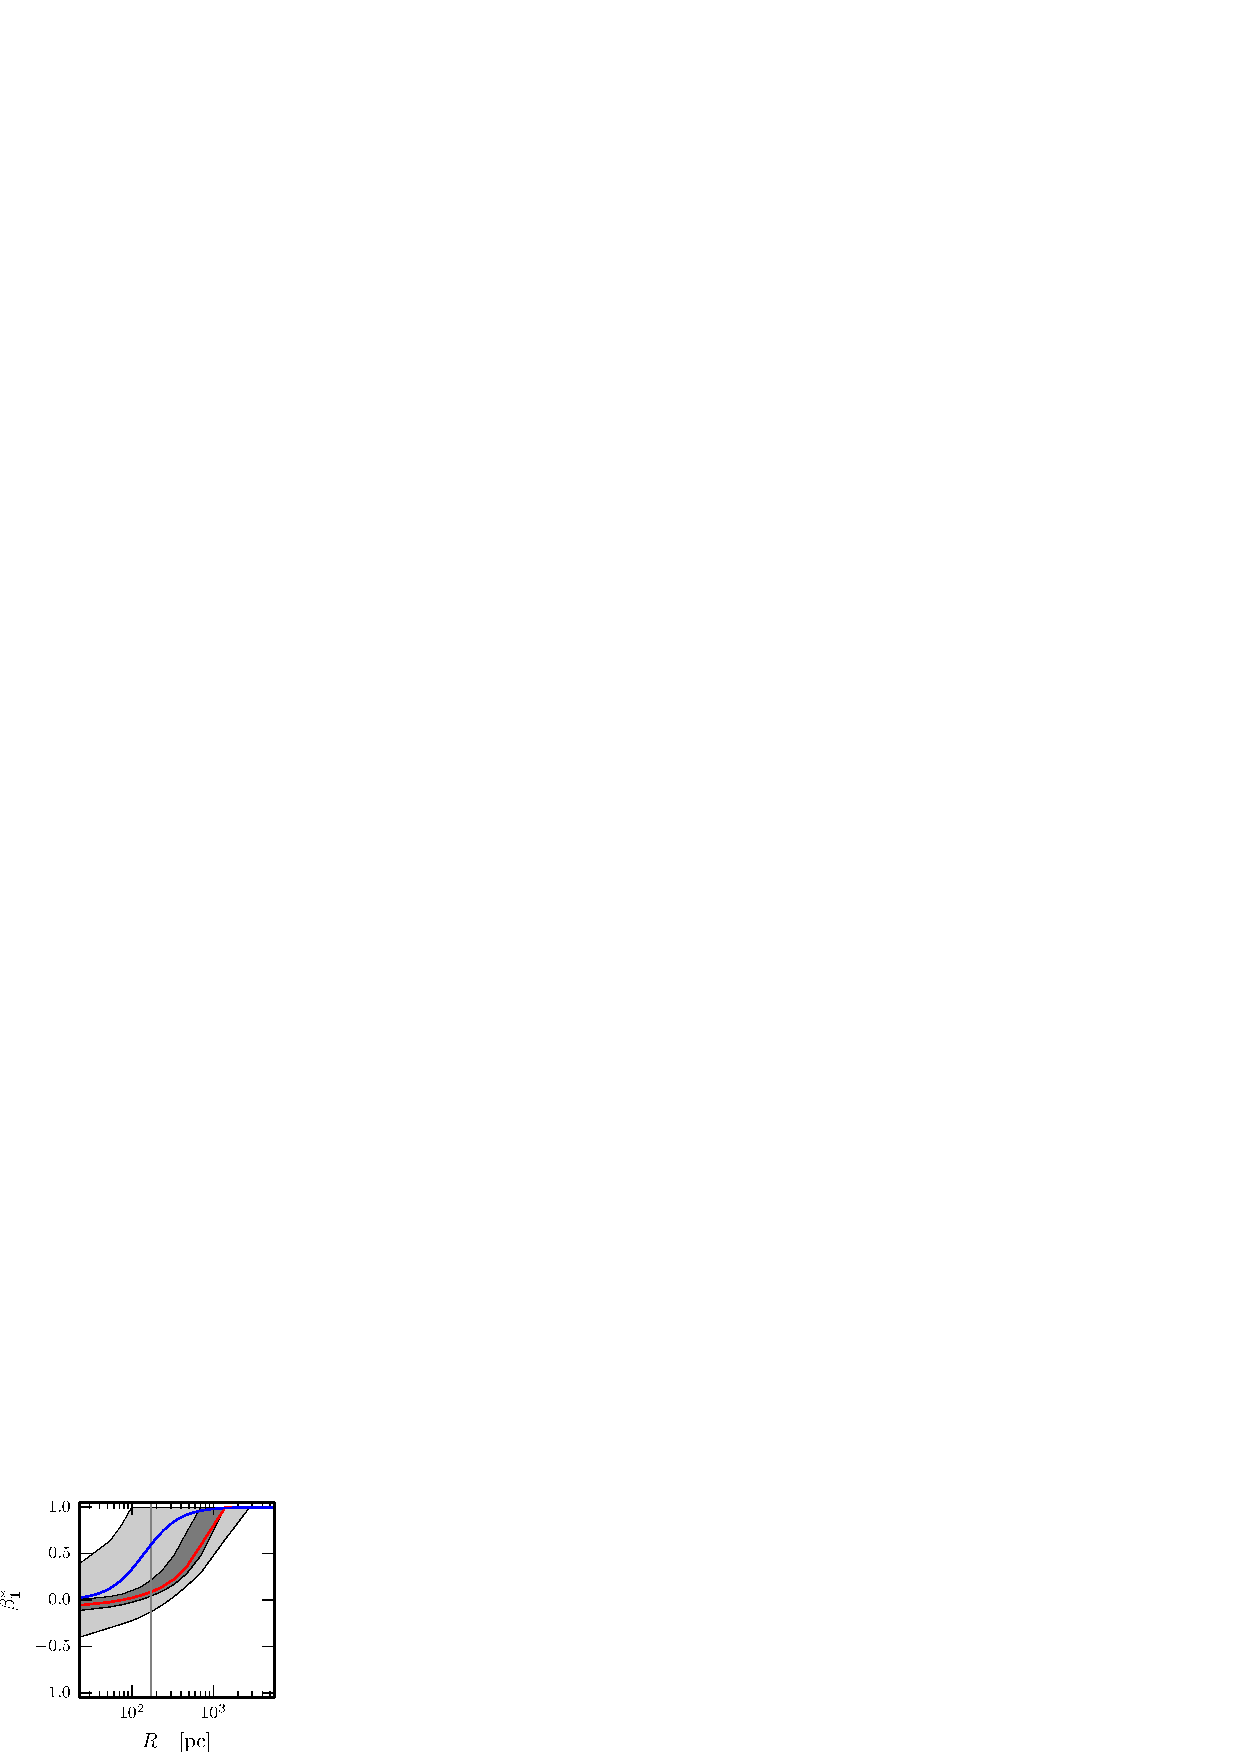
\includegraphics[width=0.3\textwidth]{fig/prof_1_pop_cusp/prof_betastar_1.png}
        \caption{Reconstructed density, density slope, and velocity
          anisotropy of a cusped model (red shows median, shaded areas
          are 68 and 95 percentiles) for $10^4$ tracer particles, for
          $3\cdot10^5$ models. The blue curve shows the underlying
          theoretical model. The half-light radius of all stellar
          tracer particles is depicted as gray vertical line.}
        \label{fig:cusp1pop}
    \end{center}
\end{figure*}

The shown plots depict the 95 and 68 confidence level (light and dark
shaded areas) and the median of all accepted models. The number of
models is equal to the number of live points in MultiNest, and is set
to twice the number of dimensions, $2\cdot N_{\rm dim}$.

% nu and sigma: fit to data
The reconstructed profiles for tracer surface density $\Sigma(r)$ and
velocity dispersion $\siglos(r)$ are shown in fig. \ref{fig:Sigsiglos1pop}.

\begin{figure*}
    \begin{center}
        \hspace{-7mm}
        \includegraphics[width=0.3\textwidth]{fig/prof_1_pop_cusp/prof_Sig_1.pdf}
        \includegraphics[width=0.3\textwidth]{fig/prof_1_pop_cusp/prof_sig_1.pdf}
        \caption{\label{fig:Sigsiglos1pop} Tracer surface density profile
          $\Sigma(r)$, normalized to 1 at $r_{1/2}$ and velocity
          dispersion profile $\siglos(r)$ for the stellar components
          in the cusped profile of fig. \ref{fig:cusp1pop}.}
    \end{center}
\end{figure*}

The original data is given as a blue shaded region. $\chi^2$ is
calculated from the difference between each model's $\Sigma(r)$ and
$\sigma_p(r)$, thus the fact that most models are consistent within
errors to the data is expected from the low $\chi^2 \leq5$ found after
some 1000 iterations.

% Introducing $\kappa_i$ in the $\chi^2$ did \TODO{not?} result in a
% change of behavior for the velocity anisotropy parameter.

\TODO{observations for kurtosis}
\TODO{link to Tom's papers: kappa does not resolve density/anisotropy degeneracy,  Virial Shape Parameters do}
\TODO{better/worse fitting of density}

\subsection{Two populations}
The same mock dwarf is analyzed with a model where both populations of
tracer particles are accounted for. This is done in the following
manner: Each particle in the mock dataset has a number identifying it
as a member of population 1, 2, or background. For the plot
\ref{fig:cusp2pop}, we used this information directly.

\begin{figure*}
    \begin{center}
        \hspace{-7mm}
        \includegraphics[width=0.3\textwidth]{fig/prof_2_pop_cusp/prof_rho_0.pdf}
        \includegraphics[width=0.3\textwidth]{fig/prof_2_pop_cusp/prof_nr_0.pdf}
        \caption{Reconstructed density and density slope for the same
          cusped model (red shows median, shaded areas are 68 and 95
          percentiles) for $2\cdot 5000$ tracer particles, for
          $3\cdot10^5$ models. The blue curve shows the underlying
          theoretical model. The half-light radii of the two
          populations of tracer particles is depicted as gray vertical
          lines.}
        \label{fig:cusp2pop}
    \end{center}
\end{figure*}

For real data, we will use a splitting based on metallicity. It has
been shown for several dwarfs (\TODO{cite Walker}) that two or more
dynamically distinct populations (\TODO{what does this mean? how can
we tell one star to be in the right population?}) of stars can be
extracted via their metallicity content.

This is achieved by using a separate Markov Chain Monte Carlo
method. The overall metallicity distribution is represented by a sum
of two Gaussians with means $\mu_{1,2}$ and widths $\sigma_{1,2}$, and
each stellar tracer with metallicity $M$ is assigned a population
based on the likelihood of its metallicity belonging to said
population. The process is repeated to marginalize over the means and
widths of the metallicity distributions. A sample splitting result is
shown in fig. \ref{fig:pymcmetal}.

\begin{figure}
    \begin{center}
        \hspace{-7mm}
        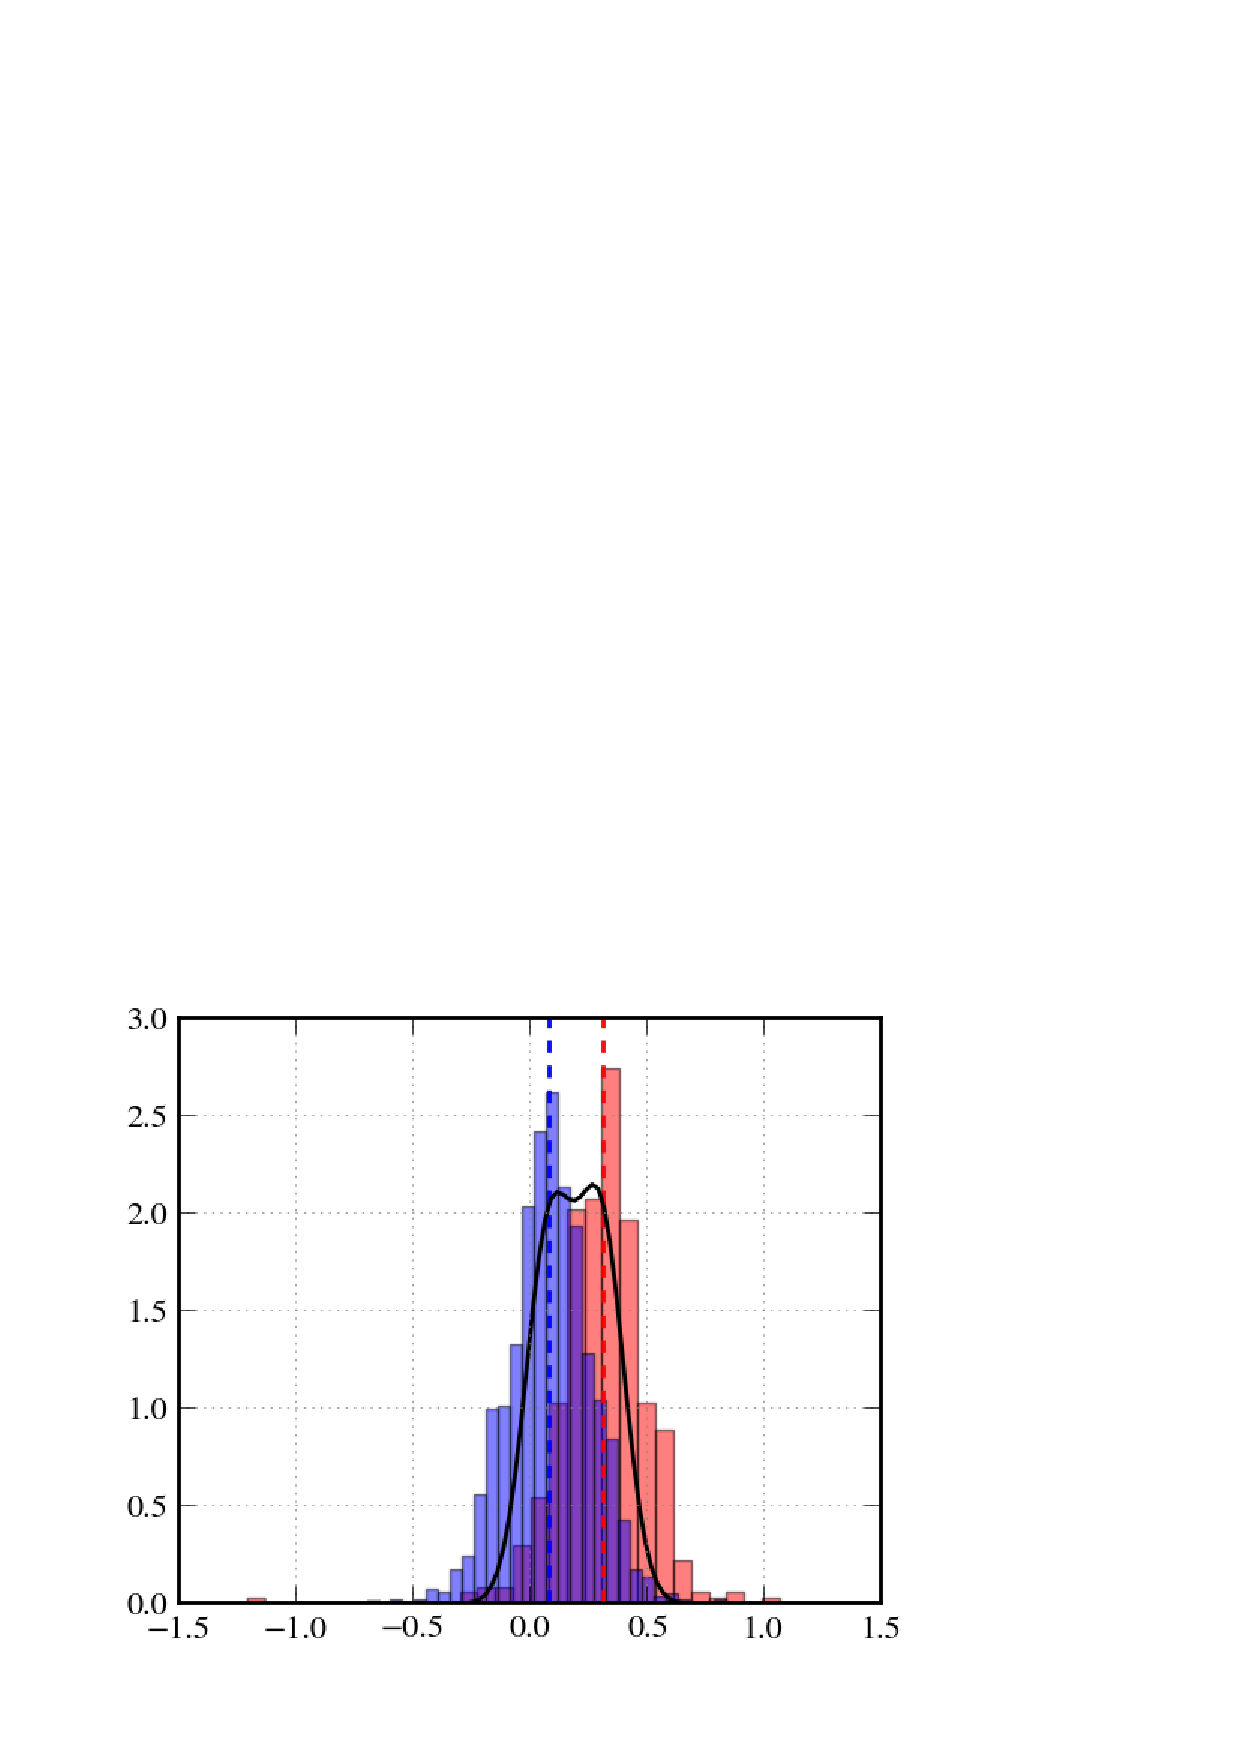
\includegraphics[width=0.5\textwidth]{fig/pymcmetals.png}
        \caption{Reconstruction of two populations from mock data. The
          underlying metallicity distributions are shown as red and
          blue histograms. The retrieved centers of the Gaussians are
          shown as vertical lines, and the reconstructed metallicity
          distribution is depicted as black line.}
        \label{fig:pymcmetal}
    \end{center}
\end{figure}

\TODO{priors} \TODO{3 populations?}

\subsection{Cored Model}
For a cored profile, with $\gamma_{\rm DM}=0$, we get the results in
fig. \ref{fig:core}.

\begin{figure*}
    \begin{center}
        \hspace{-7mm}
        % \includegraphics[width=0.3\textwidth]{fig/prof_2_pops_core/prof_rho_0.pdf}
        % \includegraphics[width=0.3\textwidth]{fig/prof_2_pops_core/prof_rho_0.pdf}
        \caption{A cored profile: Reconstructed mass of the MCMC model
          (red shows median, shaded areas are 68 and 90 percentiles)
          for $10^4$ tracer particles based on $3\cdot10^5$ sampled
          models. The blue curve shows the underlying theoretical
          model.}
        \label{fig:core}
    \end{center}
\end{figure*}


\subsection{Triaxial mock data}
To test the dependency of {\sc Gravlite} on the assumption of
spherical symmetry, we employ it on slightly triaxial mock dwarf
galaxies.

The models were generated with the Made2Measure algorithm of
\cite{Dehnen2009} and are tailored to follow a similar profile to the
profiles specified above for the dwarf galaxies. They show a density
profile of

\begin{equation}
    \rho(r)=\frac{\rho_S}{\left(\frac{r}{r_S}\right)^\gamma\left(1+\left(\frac{r}{r_S}\right)^{1/\alpha}\right)^{\alpha(\beta-\gamma)}}
\end{equation}

with radius $r$, scale radius $r_S=1.5\kpc$, $\alpha=1$,
$\beta=4$. For the cusped profiles we have an inner logarithmic slope
of $\gamma=1$, scale density $\rho_S=5.522\cdot 10^7M_\odot/\kpc^3$,
and $M_{\tot}=1.171\cdot10^9M_\odot$, while for the cored one we have
$\gamma=0.23$, $\rho_S=1.177\cdot10^8M_\odot$,
$M_{\tot}=1.802\cdot10^9M_\odot$. The axis ratios are $b/a=0.8$ and
$c/a=0.6$. The stars have negligible mass and follow the same
functional form in the density profile as dark matter, with
$\alpha=0.34, \beta=5.92, \gamma=0.23, r_S=0.81\kpc$.

The velocity anisotropy of the stellar part is calculated via

\begin{equation}
    \beta(r)=\frac{r_{s,\beta}^\eta \beta_0+r^\eta \beta_\infty}{r^\eta+r_{s,\beta}^\eta},
\end{equation}

with $r_{s,\beta}=0.81\kpc$, $\beta_0=0$, $\beta_\infty=0.5$ and
$\eta=0.5$, going from isotropic to radially anisotropic with
increasing radius.

\begin{figure*}
    \begin{center}
        \hspace{-7mm}
        \includegraphics[width=0.3\textwidth]{fig/prof_1_pop_triax/prof_rho_0.pdf}
        \includegraphics[width=0.3\textwidth]{fig/prof_1_pop_triax/prof_nr_0.pdf}
        \caption{Density profile of a triaxial mock dwarf, for which
          the line of sight is inclined with 45 degrees with respect
          to all axes. The vertical line indicates the half-light
          radius at 640pc.}
        \label{fig:triax}
    \end{center}
\end{figure*}

The retrieved density profile (fig. \ref{fig:triax}) recaptures the
density inside the half-light radius, but constantly overestimates it
at $r>r_{1/2}$. This is partly due to projection effects, as the
underlying density profile in blue is calculated for spherically
averaged density decrease.

\section{Conclusions}\label{sec:conclusions}

The new non-parametric method samples the profiles of the overall
density bin-wise, and was shown to reconstruct the density of diverse
mock data.


%%% Local Variables:
%%% mode: latex
%%% TeX-master: "Steger+_2014_Fornax"
%%% End:

\section{Acknowledgements}
JIR would like to acknowledge support from SNF grant PP00P2\_128540/1.


\bibliographystyle{mn2e}
\bibliography{thesis}

\section{Appendix}

\subsection{Effect of Wrong Assignment of Populations}
We quantify the influence of assigning stars the wrong population by
looking at the changes for

\begin{enumerate}
\item assigning stars randomly to two population
\item assigning stars to populations based on position information
  only
\end{enumerate}

\TODO{result}

\subsection{Priors in use}
We use the priors outlined in \citep{Steger+2014}, with numerical
values in table \ref{tab:priors}:

\begin{enumerate}
  \item $\beta^*(r)$ is given in the form
    \begin{equation}\label{eqn:betastar}
      \beta^* = \frac{\sigma_r^2-\sigma_t^2}{\sigma_r^2+\sigma_t^2} = \frac{\beta}{2-\beta} \in [-1,1]
    \end{equation}
    with the following function:

    \begin{eqnarray} \label{eqn:nonparabetstar}
      \beta^*(r) &=& \frac{a_0-a_\infty}{1+\kappa \exp(\alpha\ln(r/r_s))}+a_\infty\\
      \kappa &=& \frac{a_0-a_\infty}{\beta^*(r_s)-a_\infty}-1
    \end{eqnarray}


  \item $n(r)=-{\rm d}\ln\rho(r)/{\rm d}\ln r$ is calculated by integrating its
    derivative $dn(r)/d\ln r$ -- which is given at discrete bin
    centers, and drawn from a Gaussian prior of width $\sigma$ -- with
    the additional constraint that $n(r)\geq0$. The density profile

    \begin{equation*}
      \rho(r) = \rho_{1/2}\cdot\exp\left[-\int_{\ln r_{1/2}}^{\ln r}n(s)\text{d}s\right],
    \end{equation*}

    is thus represented by its second derivatives. This enforces a
    monotonically decreasing $\rho(r)$, and further circumvents strong
    oscillations from numerical effects.

  \item no use of fourth order moments $\kappa$
  \item no use of virial parameters $\zeta_A, \zeta_B$
\end{enumerate}



\begin{table}
  \label{tab:priors}
  \caption{Priors for the \GravImage method used on Fornax.}
  \centering
  \begin{tabular}{lllll}
    Quantity & type & characteristics \\
    \hline
    $N_{bin}$ & fixed & 12\\
    $n_\beta$ & fixed & 4\\
    $dn(r)/d\ln r$ & Gaussian & mean 0, width $\sigma=5$\\
    $n(r)$ & bound & $\min(n(r))=0$\\
    $\ln \rho(r_{1/2})$ & flat & center $-1$, width $2.5$ dex\\
    $M/L$ & flat & $[0.8, 3]$
  \end{tabular}
\end{table}



%%% Local Variables:
%%% mode: latex
%%% TeX-master: "Steger+_2014_Fornax"
%%% End:


\end{document}
